\section{Casi d'uso}
\subsection{Introduzione}
In questa sezione vengono presentati i casi d'uso individuati durante l'attività di analisi, 
condotta a partire dal capitolato d'appalto e dagli incontri con il proponente. 
Gli attori vengono identificati in base alla gerarchia trovata e 
alle funzionalità potenziali rilevate.

\subsubsection{Codifica dei casi d'uso}
I casi d'uso sono codificati utilizzando la seguente notazione:

\begin{itemize}
    \item \textbf{UC[ID-Principale][ID-Sottocaso]}: Identificativo univoco del caso d'uso, composto da un ID principale che identifica il caso principale e, se necessario, da un ID del sottocaso.
    \item \textbf{Titolo}: Breve descrizione del caso d'uso.
    \item \textbf{Attori}: Elenco degli attori coinvolti nel caso d'uso.
    \item \textbf{Precondizioni}: Condizioni che devono essere vere prima che il caso d'uso possa iniziare.
    \item \textbf{Postcondizioni}: Condizioni che devono essere vere dopo che il caso d'uso è stato completato con successo.
    \item \textbf{Scenario principale}: Descrizione dettagliata del flusso di eventi principale del caso d'uso.
    \item \textbf{Generalizzazioni}: Eventuali casi d'uso generalizzati.
    \item \textbf{Estensioni}: Eventuali casi d'uso estesi.
    \item \textbf{Inclusione}: Eventuali inclusioni.
\end{itemize}
\newpage
\subsection{Elenco dei Casi d'uso}

\subsubsection{U.C.1 Scrivi Messaggio}
\begin{itemize}
    \item \textbf{Attore}: Utente
    \item \textbf{Precondizioni}: Utente che ha acceduto nel sistema e vuole domandare al bot delle informazioni riguardo un prodotto o una serie di prodotti
    \item \textbf{Postcondizioni}: L'utente ha inviato il messaggio al bot per ricevere una risposta.  
    \item \textbf{Scenario principale}: L’utente apre la chat, inserisce la domanda nella casella di testo e invia il messaggio premendo il pulsante ”Invia”.
    \item \textbf{Generalizzazioni}: -
    \item \textbf{Estensioni}: -
    \item \textbf{Inclusione}: -
\end{itemize}
\begin{figure}[H]
    \centering
    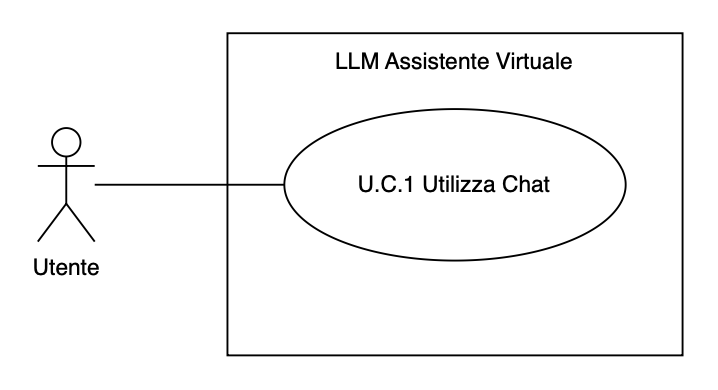
\includegraphics[width=0.7\textwidth]{img/UC1.png}
    \caption{U.C.1 Scrivi Messaggio}
\end{figure}
\newpage

\subsubsection{U.C.2 Visualizza Risposta}
\begin{itemize}
    \item \textbf{Attore}: Utente
    \item \textbf{Attore Secondario}: OpenAi
    \item \textbf{Precondizioni}:  L'utente ha inviato una domanda al bot e attende una risposta.
    \item \textbf{Postcondizioni}: Utente riceve una risposta dal bot coerente alla domanda che ha effettuato.
    \item \textbf{Scenario principale}:  Dopo aver inviato una domanda, l'utente attende la risposta elaborata dall’\href{https://code7crusaders.github.io/docs/RTB/documentazione_interna/glossario.html#llm-large-language-model}{\textit{LLM}\textsuperscript{G}} che viene visualizzata nella finestra della chat.
    \item \textbf{Generalizzazioni}: -
    \item \textbf{Estensioni}: U.C.2.1
    \item \textbf{Inclusione}: -
\end{itemize}
\begin{figure}[H]
    \centering
    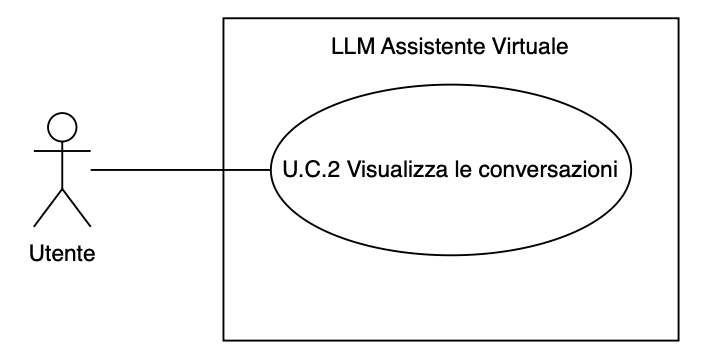
\includegraphics[width=0.8\textwidth]{img/UC2.png}
    \caption{U.C.2 Visualizza Risposta}
\end{figure}
\newpage

\subsubsection{U.C.2.1 Prodotto non trovato}
\begin{itemize}
    \item \textbf{Attore}: Utente
    \item \textbf{Precondizioni}: L'utente richiede informazioni su un prodotto non presente nel database del sistema.
    \item \textbf{Postcondizioni}: L'utente riceve una risposta da parte del \href{https://code7crusaders.github.io/docs/RTB/documentazione_interna/glossario.html#llm-large-language-model}{LLM\textsuperscript{G}}, non è possibile elaborare l'informazione.
    \item \textbf{Scenario principale}: L'utente invia una domanda su un prodotto specifico, il sistema cerca nel database ma non trova risultati. Un messaggio di errore avvisa l'utente che il prodotto 
    \item \textbf{Generalizzazioni}: -
    \item \textbf{Estensioni}: -
    \item \textbf{Inclusione}: -
\end{itemize}
\begin{figure}[H]
    \centering
    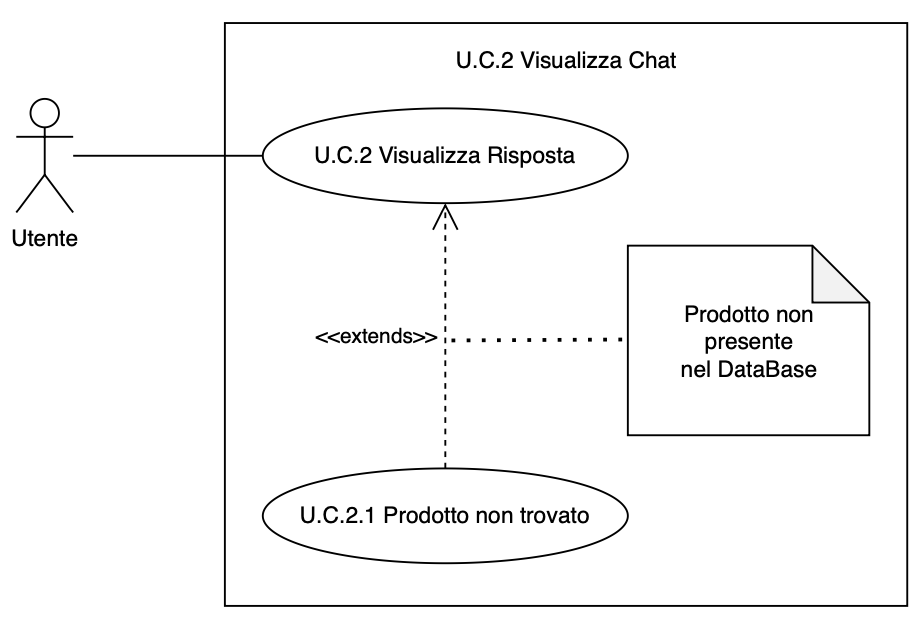
\includegraphics[width=0.7\textwidth]{img/UC2.1.png}
    \caption{U.C.2.1 Prodotto non Trovato}
\end{figure}
\newpage
 
\subsubsection{U.C.3 Seleziona Template}
\begin{itemize}
    \item \textbf{Attore}: Utente
    \item \textbf{Precondizioni}: L'utente ha effettuato l'accesso ed è nella chat. Vuole selezionare una domanda predefinita tra quelle suggerite dal sistema. 
    \item \textbf{Postcondizioni}: L'utente riceve una risposta templatizzata senza dover formulare una domanda manuale.(senza dover chiamare l’\href{https://code7crusaders.github.io/docs/RTB/documentazione_interna/glossario.html#llm-large-language-model}{\textit{LLM}\textsuperscript{G}}).
    \item \textbf{Scenario principale}: L'utente visualizza un elenco di domande suggerite, ne seleziona una e il sistema fornisce immediatamente una risposta.
    \item \textbf{Generalizzazioni}: -
    \item \textbf{Estensioni}: -
    \item \textbf{Inclusione}: -
\end{itemize}
\begin{figure}[H]
    \centering
    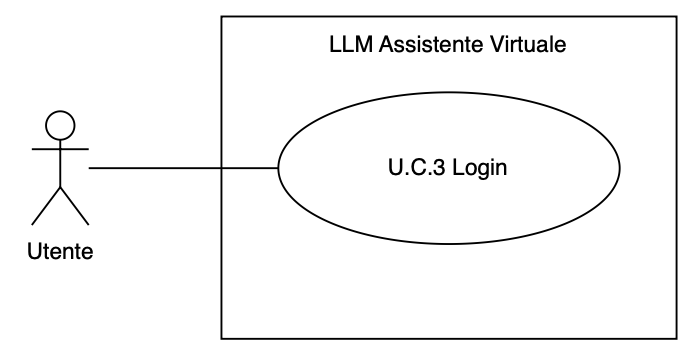
\includegraphics[width=0.7\textwidth]{img/UC3.png}
    \caption{U.C.3 Seleziona Template}
\end{figure}
\newpage

\subsubsection{U.C.4 Visualizza lista conversazioni precedenti}
\begin{itemize}
    \item \textbf{Attore}: Utente
    \item \textbf{Precondizioni}: L'utente ha effettuato l'accesso e in passato ha salvato almeno una conversazione.
    \item \textbf{Postcondizioni}: L'utente visualizza l'elenco delle conversazioni salvate.
    \item \textbf{Scenario principale}: L'utente accede alla sezione delle conversazioni e visualizza una lista ordinata delle sue conversazioni passate.
    \item \textbf{Generalizzazioni}: -
    \item \textbf{Estensioni}: -
    \item \textbf{Inclusione}: -
\end{itemize}
\begin{figure}[H]
    \centering
    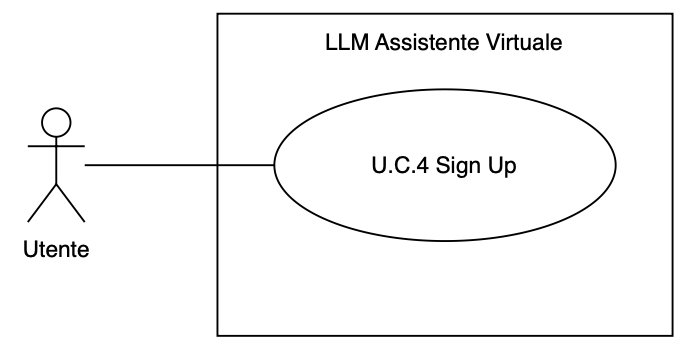
\includegraphics[width=0.7\textwidth]{img/UC4.png}
    \caption{U.C.4 Visualizza lista conversazioni precedenti}
\end{figure}
\newpage

\subsubsection{U.C.5 Visualizza Singola Conversazione Precedente}
\begin{itemize}
    \item \textbf{Attore}: Utente
    \item \textbf{Precondizioni}: L'utente ha effettuato l'accesso e in passato ha salvato almeno una conversazione.
    \item \textbf{Postcondizioni}: L'utente visualizza una conversazione salvata.
    \item \textbf{Scenario principale}: L'utente accede alla sezione delle conversazioni e visualizza una delle sue conversazioni passate.
    \item \textbf{Generalizzazioni}: -
    \item \textbf{Estensioni}: -
    \item \textbf{Inclusione}: -
\end{itemize}
\begin{figure}[H]
    \centering
    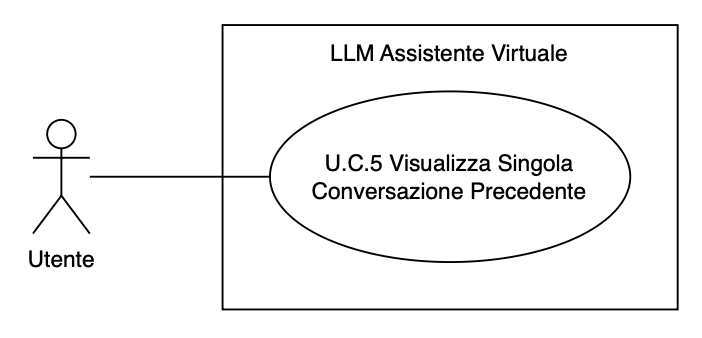
\includegraphics[width=0.7\textwidth]{img/UC5.png}
    \caption{U.C.5 Visualizza Singola Conversazione Precedente}
\end{figure}
\newpage

\subsubsection{U.C.6 Login}
\begin{itemize}
    \item \textbf{Attore}: Utente
    \item \textbf{Precondizioni}: L'utente è registrato e desidera accedere al sistema.
    \item \textbf{Postcondizioni}: L'utente accede con successo al sistema e può utilizzare le funzionalità disponibili.
    \item \textbf{Scenario principale}: L'utente inserisce il proprio username e password nei campi di accesso ed effettua l’accesso. Il sistema verifica le credenziali e consente l'accesso.  
    \item \textbf{Generalizzazioni}: -
    \item \textbf{Estensioni}: -
    \item \textbf{Inclusione}: U.C.6.1, U.C.6.2
\end{itemize}
\begin{figure}[H]
    \centering
    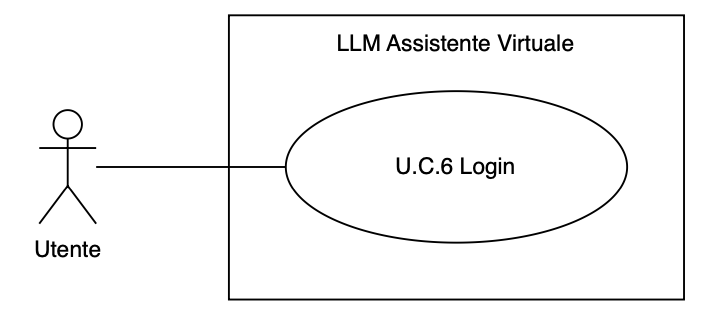
\includegraphics[width=0.7\textwidth]{img/UC6.png}
    \caption{U.C.6 Login}
\end{figure}
\newpage

\subsubsection{U.C.6.1 Inserisci Username}
\begin{itemize}
    \item \textbf{Attore}: Utente
    \item \textbf{Precondizioni}: L'utente desidera accedere al sistema.
    \item \textbf{Postcondizioni}: L'username è stato inserito correttamente nel campo corrispondente.
    \item \textbf{Scenario principale}: L'utente digita il proprio username nel campo di testo dedicato e procede con l'autenticazione.
    \item \textbf{Generalizzazioni}: -
    \item \textbf{Estensioni}: U.C.6.4, U.C.6.5
    \item \textbf{Inclusione}: -
\end{itemize}
\begin{figure}[H]
    \centering
    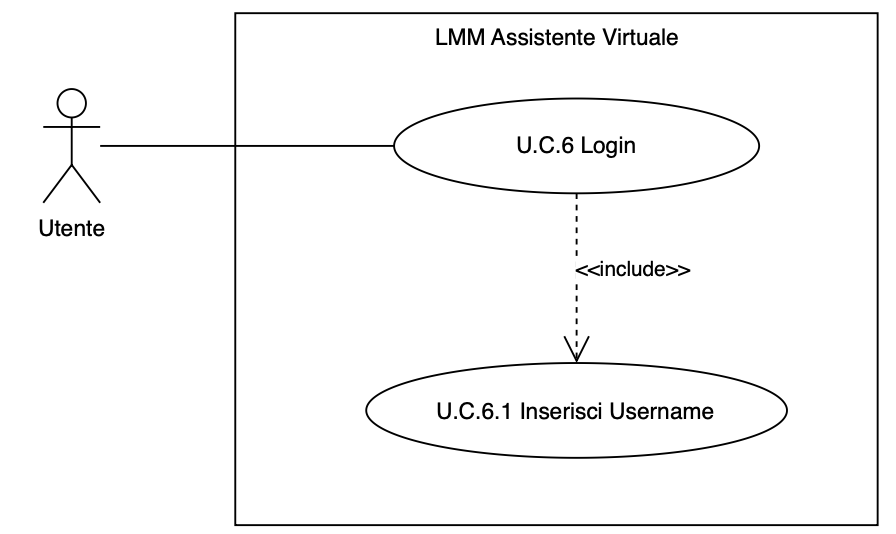
\includegraphics[width=0.8\textwidth]{img/UC6.1.png}
    \caption{U.C.6.1 Inserisci Username}
\end{figure}
\newpage

\subsubsection{U.C.6.2 Inserisci Password}
\begin{itemize}
    \item \textbf{Attore}: Utente
    \item \textbf{Precondizioni}: L'utente desidera accedere al sistema.
    \item \textbf{Postcondizioni}: La password è stata inserita correttamente nel campo corrispondente.
    \item \textbf{Scenario principale}: L'utente digita la password nel campo di testo e procede con l'autenticazione.
    \item \textbf{Generalizzazioni}: -
    \item \textbf{Estensioni}: U.C.6.3, U.C.6.5
    \item \textbf{Inclusione}: -
\end{itemize}
\begin{figure}[H]
    \centering
    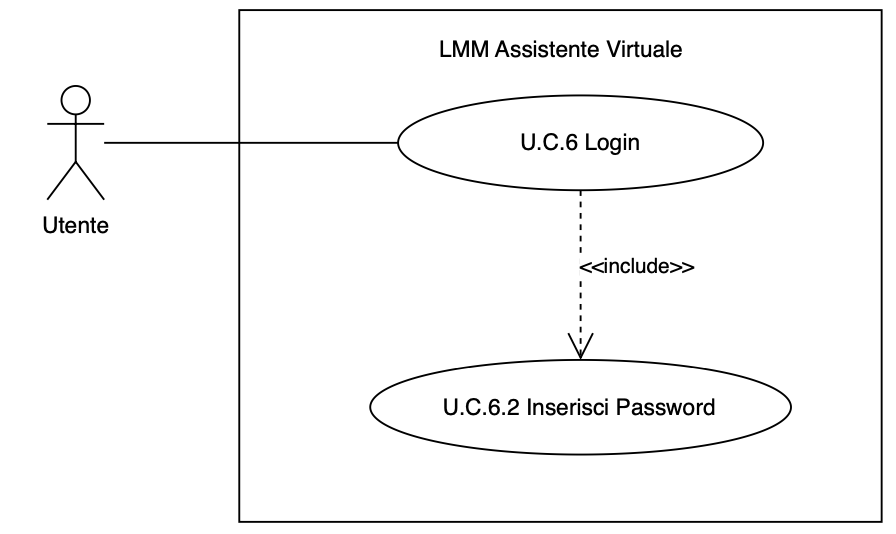
\includegraphics[width=0.8\textwidth]{img/UC6.2.png}
    \caption{U.C.6.2 Inserisci Password}
\end{figure}
\newpage

\subsubsection{U.C.6.3 Password Errata}
\begin{itemize}
    \item \textbf{Attore}: Utente
    \item \textbf{Precondizioni}: L'utente ha inserito una password non corrispondente a quella registrata.
    \item \textbf{Postcondizioni}: L'accesso viene negato e il sistema visualizza un messaggio di errore.
    \item \textbf{Scenario principale}: L'utente inserisce una password sbagliata. Il sistema verifica le credenziali, rileva l'errore e mostra un messaggio che informa l'utente dell'errore.
    \item \textbf{Generalizzazioni}: -
    \item \textbf{Estensioni}: -
    \item \textbf{Inclusione}: -
\end{itemize}
\begin{figure}[H]
    \centering
    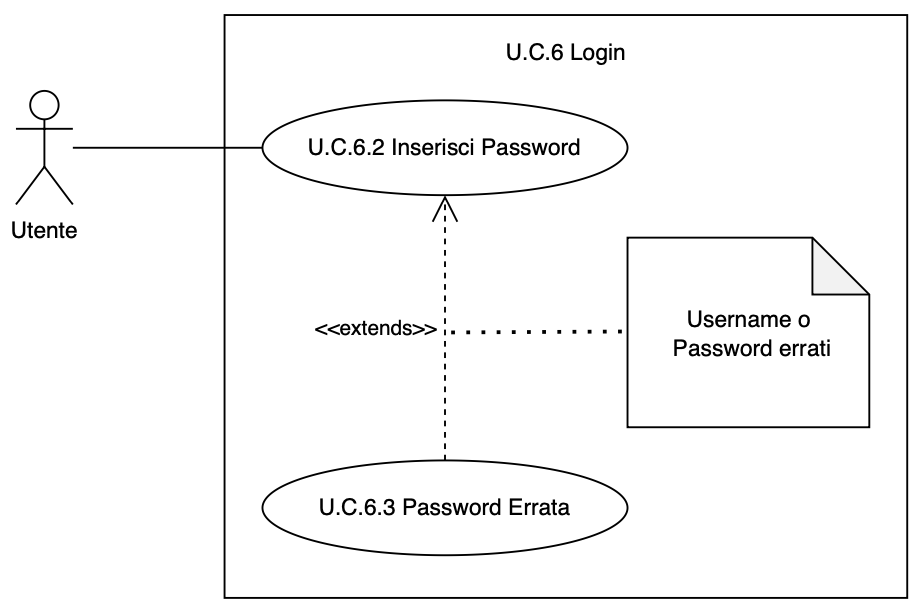
\includegraphics[width=0.8\textwidth]{img/UC6.3.png}
    \caption{U.C.6.3 Password Errata}
\end{figure}
\newpage

\subsubsection{U.C.6.4 Username Errato}
\begin{itemize}
    \item \textbf{Attore}: Utente
    \item \textbf{Precondizioni}: L'utente ha inserito un username non registrato o con errori di battitura.
    \item \textbf{Postcondizioni}: L'accesso viene negato e il sistema visualizza un messaggio di errore.
    \item \textbf{Scenario principale}: L'utente digita un username inesistente. Il sistema verifica i dati e notifica l'errore.
    \item \textbf{Generalizzazioni}: -
    \item \textbf{Estensioni}: -
    \item \textbf{Inclusione}: -
\end{itemize}
\begin{figure}[H]
    \centering
    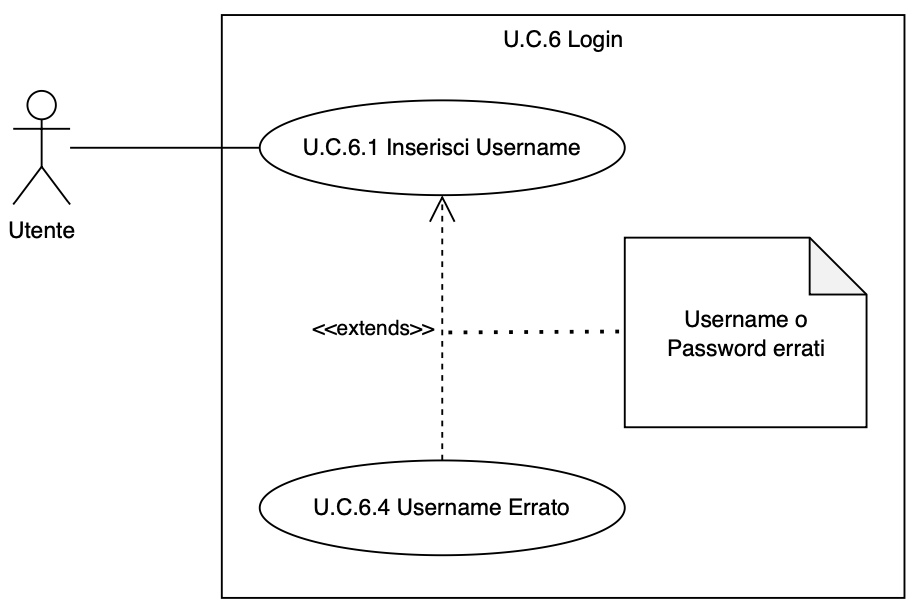
\includegraphics[width=0.8\textwidth]{img/UC6.4.png}
    \caption{U.C.6.4 Username Errato}
\end{figure}
\newpage

\subsubsection{U.C.6.5 Caratteri non Validi}
\begin{itemize}
    \item \textbf{Attore}: Utente
    \item \textbf{Precondizioni}: L'utente inserisce dati che contengono caratteri non ammessi.
    \item \textbf{Postcondizioni}: L'accesso viene negato e viene mostrato un messaggio di errore specifico.
    \item \textbf{Scenario principale}: L'accesso viene negato e viene mostrato un messaggio di errore specifico.
    \item \textbf{Generalizzazioni}: -
    \item \textbf{Estensioni}: -
    \item \textbf{Inclusione}: -
\end{itemize}
\begin{figure}[H]
    \centering
    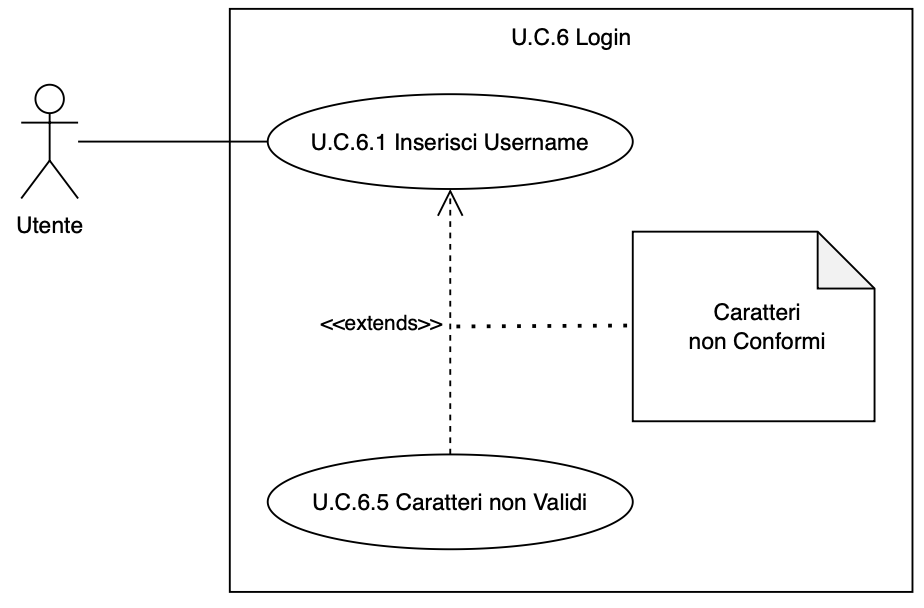
\includegraphics[width=0.6\textwidth]{img/UC6.5.1.png}
    %\caption{U.C.6.5 Caratteri non Validi}
\end{figure}
\begin{figure}[H]
    \centering
    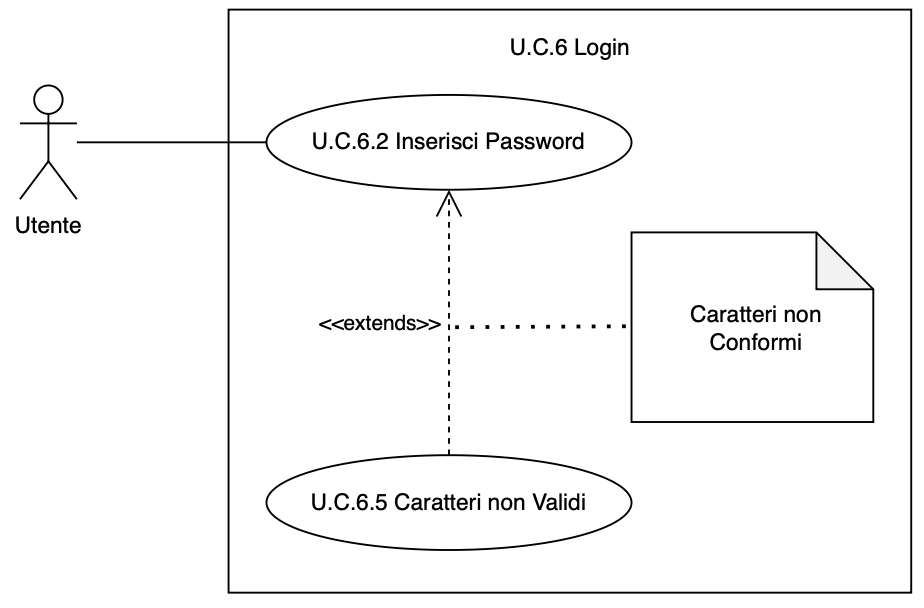
\includegraphics[width=0.6\textwidth]{img/UC6.5.2.png}
    \caption{U.C.6.5 Caratteri non Validi}
\end{figure}
\newpage

\subsubsection{U.C.7 Sign Up}
\begin{itemize}
    \item \textbf{Attore}: Utente
    \item \textbf{Precondizioni}: L'utente non è registrato al sistema e desidera accedere ai servizi.
    \item \textbf{Postcondizioni}: L'utente viene registrato con successo e può accedere al sistema.
    \item \textbf{Scenario principale}: L'utente seleziona l'opzione di registrazione, compila i campi richiesti come username e password, e conferma l'operazione. Il sistema verifica i dati e completa la registrazione.
    \item \textbf{Generalizzazioni}: -
    \item \textbf{Estensioni}: -
    \item \textbf{Inclusione}: U.C.7.1, U.C.7.2
\end{itemize}
\begin{figure}[H]
    \centering
    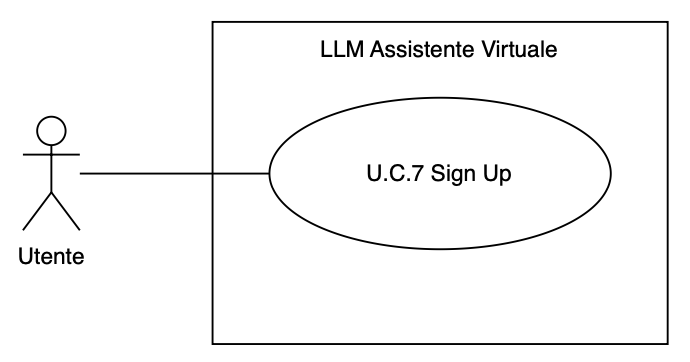
\includegraphics[width=0.7\textwidth]{img/UC7.png}
    \caption{U.C.7 Sign Up}
\end{figure}
\newpage

\subsubsection{U.C.7.1 Inserisci Username}
\begin{itemize}
    \item \textbf{Attore}: Utente
    \item \textbf{Precondizioni}: L'utente non è registrato e sta procedendo alla creazione di un account.
    \item \textbf{Postcondizioni}: L'username è stato inserito correttamente nel sistema.
    \item \textbf{Scenario principale}: L'utente compila il campo "Username" durante la registrazione e procede al passaggio successivo.
    \item \textbf{Generalizzazioni}: -
    \item \textbf{Estensioni}: -
    \item \textbf{Inclusione}: U.C.7.3, U.C.7.4, U.C.7.6
\end{itemize}
\begin{figure}[H]
    \centering
    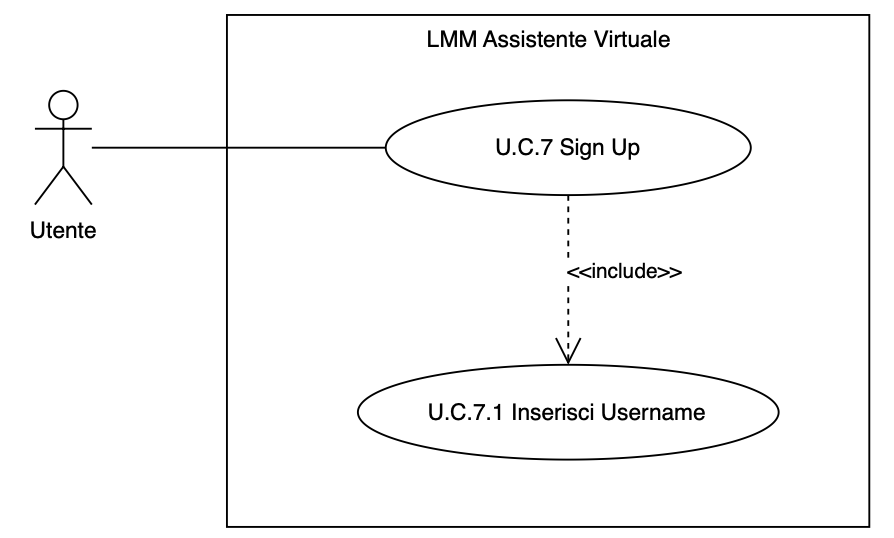
\includegraphics[width=0.8\textwidth]{img/UC7.1.png}
    \caption{U.C.7.1 Inserisci Username}
\end{figure}
\newpage

\subsubsection{U.C.7.2 Inserisci Password}
\begin{itemize}
    \item \textbf{Attore}: Utente
    \item \textbf{Precondizioni}: L'utente non è registrato e sta completando il processo di registrazione.
    \item \textbf{Postcondizioni}: La password viene salvata correttamente nel sistema.
    \item \textbf{Scenario principale}: L'utente inserisce una password nel campo corrispondente e procede con la registrazione. 
    \item \textbf{Generalizzazioni}: -
    \item \textbf{Estensioni}: -
    \item \textbf{Inclusione}: U.C.7.3, U.C.7.5
\end{itemize}
\begin{figure}[H]
    \centering
    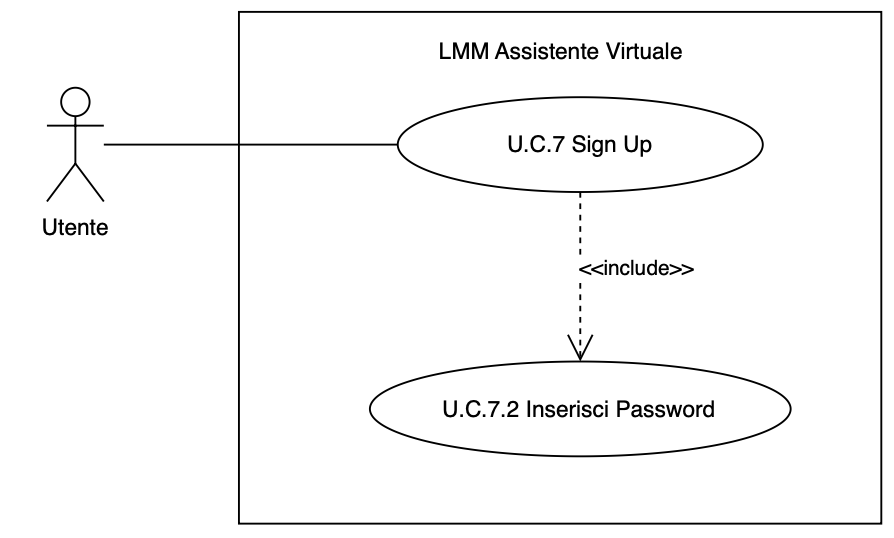
\includegraphics[width=0.8\textwidth]{img/UC7.2.png}
    \caption{U.C.7.2 Inserisci Password}
\end{figure}
\newpage

\subsubsection{U.C.7.3 Caratteri non Validi}
\begin{itemize}
    \item \textbf{Attore}: Utente
    \item \textbf{Precondizioni}: Durante la registrazione, l'utente inserisce caratteri non consentiti nel campo username o password.
    \item \textbf{Postcondizioni}: La registrazione viene interrotta e l'utente riceve un messaggio di errore.
    \item \textbf{Scenario principale}: L'utente tenta di registrarsi ma utilizza caratteri non validi nei campi obbligatori. Il sistema rileva l'errore e avvisa l'utente.
    \item \textbf{Generalizzazioni}: -
    \item \textbf{Estensioni}: -
    \item \textbf{Inclusione}: -
\end{itemize}
\begin{figure}[H]
    \centering
    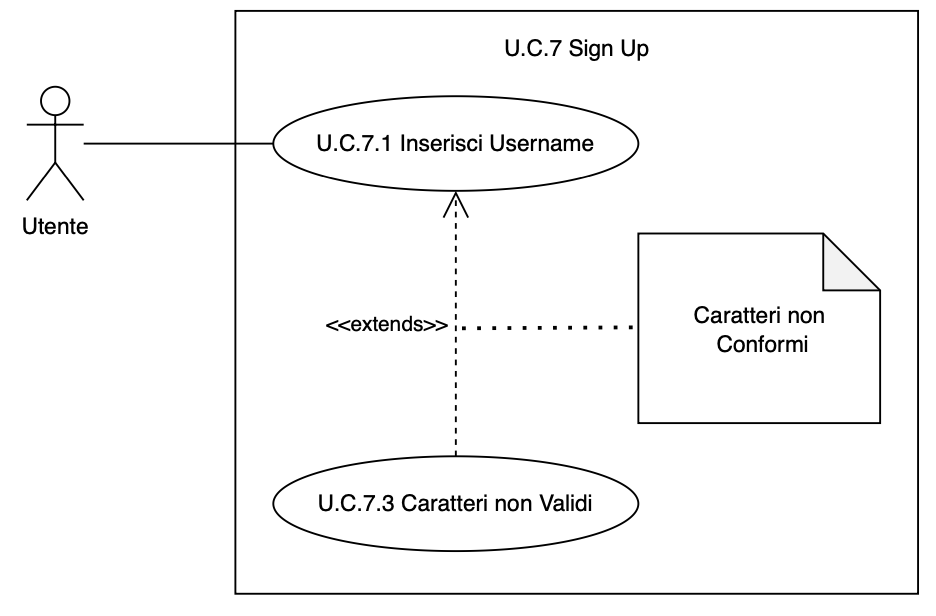
\includegraphics[width=0.6\textwidth]{img/UC7.3.1.png}
    %\caption{U.C.7.3 Caratteri non Validi}
\end{figure}
\begin{figure}[H]
    \centering
    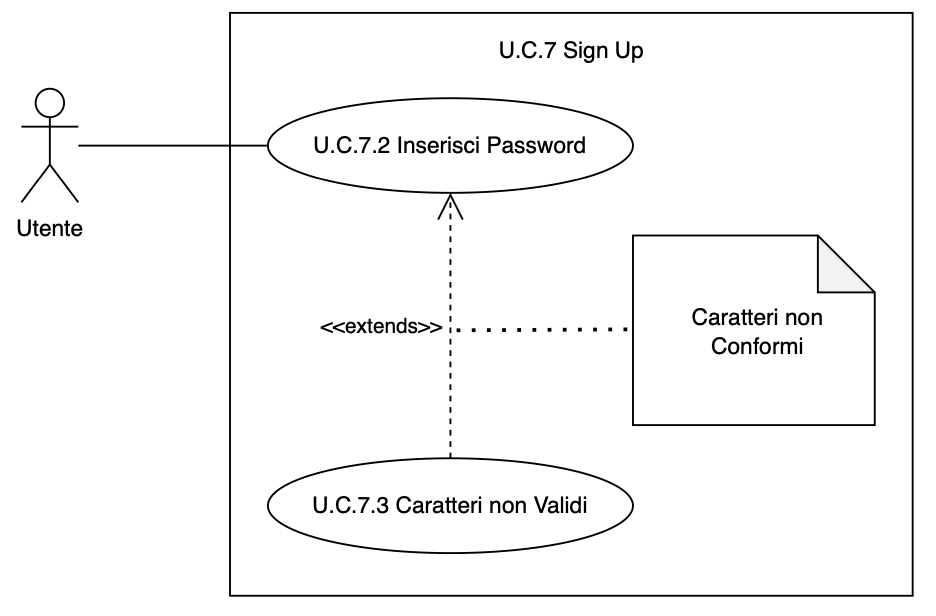
\includegraphics[width=0.6\textwidth]{img/UC7.3.2.png}
    \caption{U.C.7.3 Caratteri non Validi}
\end{figure}
\newpage

\subsubsection{U.C.7.4 Username troppo Lungo}
\begin{itemize}
    \item \textbf{Attore}: Utente
    \item \textbf{Precondizioni}: L'utente inserisce un username che supera il limite massimo di caratteri consentiti.
    \item \textbf{Postcondizioni}: La registrazione non viene completata e l'utente riceve un messaggio di errore. 
    \item \textbf{Scenario principale}: Durante la registrazione, il sistema rileva che l'username è troppo lungo e informa l'utente. 
    \item \textbf{Generalizzazioni}: -
    \item \textbf{Estensioni}: -
    \item \textbf{Inclusione}: -
\end{itemize}
\begin{figure}[H]
    \centering
    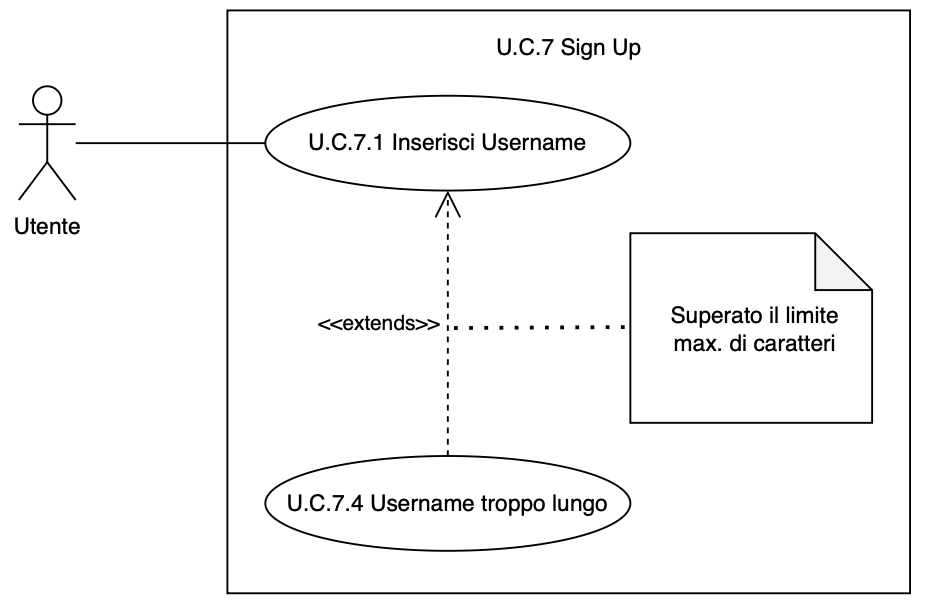
\includegraphics[width=0.8\textwidth]{img/UC7.4.png}
    \caption{U.C.7.4 Username troppo Lungo}
\end{figure}
\newpage

\subsubsection{U.C.7.5 Password troppo Lunga}
\begin{itemize}
    \item \textbf{Attore}: Utente
    \item \textbf{Precondizioni}: L'utente inserisce una password che supera il limite massimo consentito.
    \item \textbf{Postcondizioni}: La registrazione viene bloccata e l'utente viene informato dell'errore.  
    \item \textbf{Scenario principale}: L'utente tenta di completare la registrazione ma il sistema respinge la password perché troppo lunga. 
    \item \textbf{Generalizzazioni}: -
    \item \textbf{Estensioni}: -
    \item \textbf{Inclusione}: -
\end{itemize}
\begin{figure}[H]
    \centering
    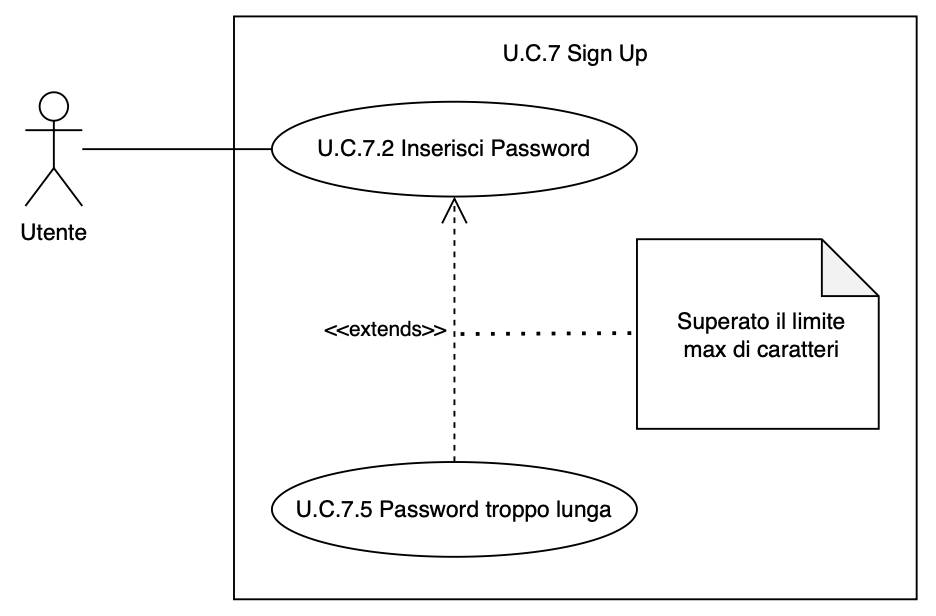
\includegraphics[width=0.8\textwidth]{img/UC7.5.png}
    \caption{U.C.7.5 Password troppo lunga}
\end{figure}
\newpage

\subsubsection{U.C.7.6 Username già presente}
\begin{itemize}
    \item \textbf{Attore}: Utente
    \item \textbf{Precondizioni}: L'utente inserisce un username già esistente nel sistema.
    \item \textbf{Postcondizioni}: La registrazione viene interrotta e il sistema suggerisce di scegliere un altro username.  
    \item \textbf{Scenario principale}: L'utente tenta di registrarsi con uno username già utilizzato e il sistema blocca l'operazione con un messaggio informativo. 
    \item \textbf{Generalizzazioni}: -
    \item \textbf{Estensioni}: -
    \item \textbf{Inclusione}: -
\end{itemize}
\begin{figure}[H]
    \centering
    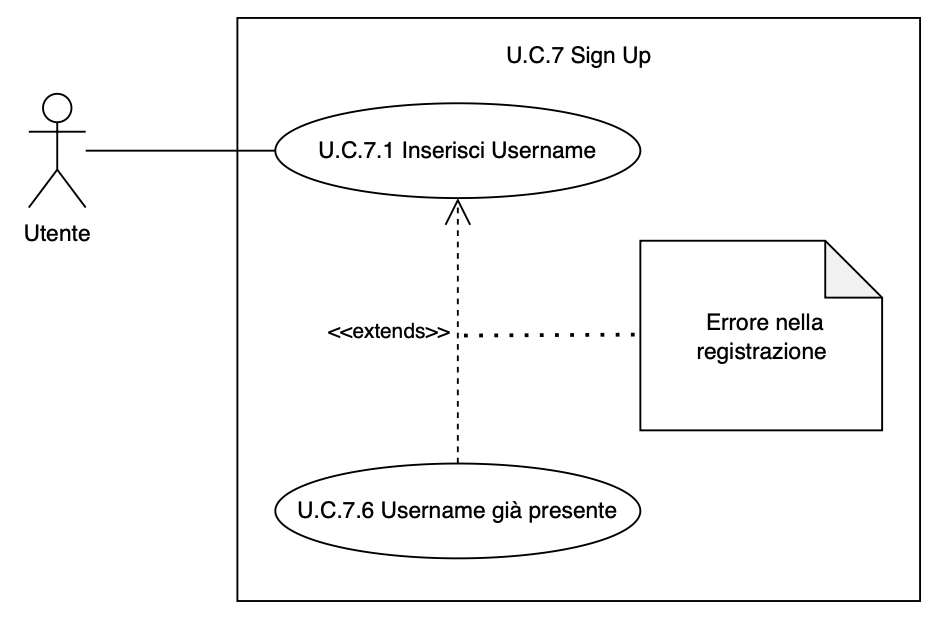
\includegraphics[width=0.8\textwidth]{img/UC7.6.png}
    \caption{U.C.7.6 Username già presente}
\end{figure}
\newpage

\subsubsection{U.C.8 Salva Chat}
\begin{itemize}
    \item \textbf{Attore}: Utente
    \item \textbf{Precondizioni}: L'utente ha completato una conversazione con il bot e desidera conservarlo per consultazioni future. 
    \item \textbf{Postcondizioni}: La conversazione viene salvata e aggiunta all'elenco delle chat salvate.
    \item \textbf{Scenario principale}: Dopo aver terminato la conversazione, l'utente seleziona l'opzione "Salva Chat" e il sistema archivia la conversazione.
    \item \textbf{Generalizzazioni}: -
    \item \textbf{Estensioni}: U.C.8.1
    \item \textbf{Inclusione}: -
\end{itemize}
\begin{figure}[H]
    \centering
    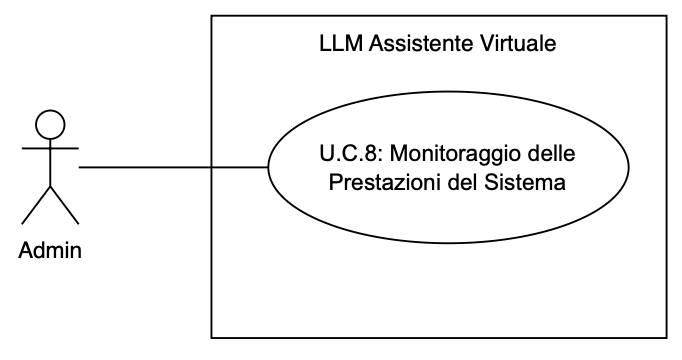
\includegraphics[width=0.7\textwidth]{img/UC8.png}
    \caption{U.C.8 Salva Chat}
\end{figure}
\newpage

\subsubsection{U.C.8.1 Memoria Piena}
\begin{itemize}
    \item \textbf{Attore}: Utente
    \item \textbf{Precondizioni}: L'utente ha superato il limite di conversazioni salvabili nel proprio account.
    \item \textbf{Postcondizioni}: La conversazione non viene salvata e l'utente riceve un avviso.
    \item \textbf{Scenario principale}: L'utente tenta di salvare una chat, ma il sistema rileva che lo spazio dedicato alle conversazioni è esaurito. Il sistema invita l'utente a eliminare alcune chat per liberare spazio.
    \item \textbf{Generalizzazioni}: -
    \item \textbf{Estensioni}: -
    \item \textbf{Inclusione}: -
\end{itemize}
\begin{figure}[H]
    \centering
    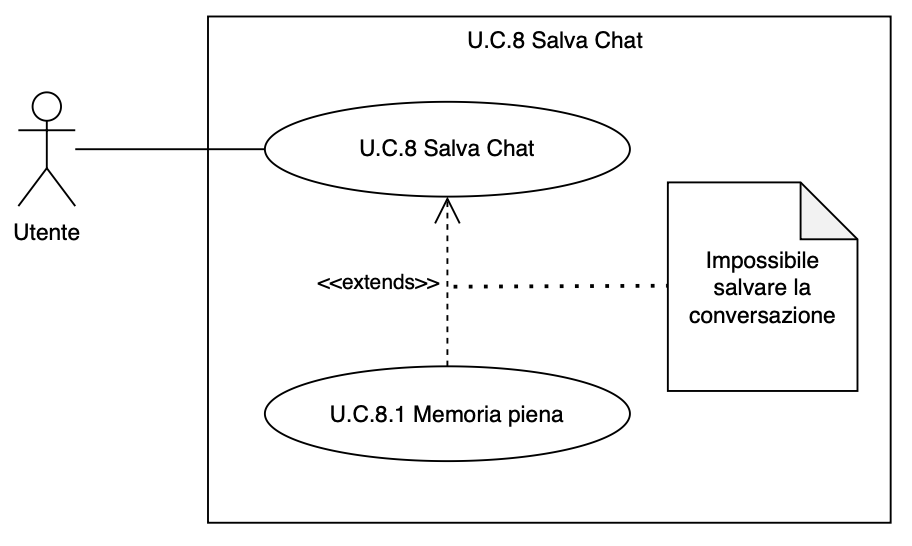
\includegraphics[width=0.8\textwidth]{img/UC8.1.png}
    \caption{U.C.8.1 Memoria Piena}
\end{figure}
\newpage

\subsubsection{U.C.9 Feedback Chat}
\begin{itemize}
    \item \textbf{Attore}: Utente
    \item \textbf{Precondizioni}: L'utente ha completato una conversazione con il bot e vuole esprimere un giudizio sulla qualità delle risposte ricevute.
    \item \textbf{Postcondizioni}: Il feedback viene registrato nel sistema per analisi future.
    \item \textbf{Scenario principale}: Dopo la conversazione, l'utente valuta il bot scegliendo un'opzione di feedback (positivo o negativo). Il sistema registra il giudizio per migliorare le prestazioni future.
    \item \textbf{Generalizzazioni}: -
    \item \textbf{Estensioni}: -
    \item \textbf{Inclusione}: -
\end{itemize}
\begin{figure}[H]
    \centering
    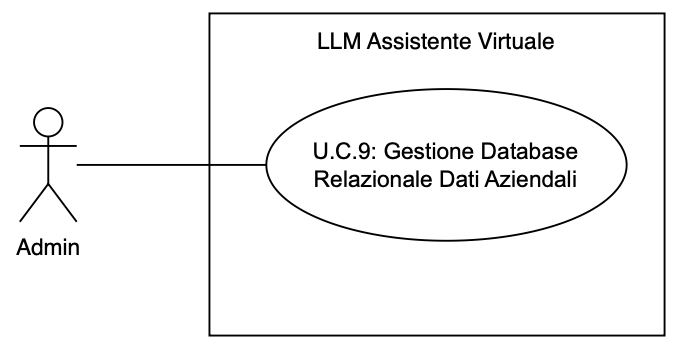
\includegraphics[width=0.7\textwidth]{img/UC9.png}
    \caption{U.C.9 Feedback Chat}
\end{figure}
\newpage

\subsubsection{U.C.10: Creazione di un nuovo template}
\begin{itemize}
    \item \textbf{Attore}: Admin
    \item \textbf{Precondizioni}: L'amministratore ha effettuato l'accesso al sistema di gestione e ha selezionato l'opzione per creare un nuovo \href{https://code7crusaders.github.io/docs/RTB/documentazione_interna/glossario.html#template}{template\textsuperscript{G}}.
    \item \textbf{Postcondizioni}: Un nuovo \href{https://code7crusaders.github.io/docs/RTB/documentazione_interna/glossario.html#template}{template\textsuperscript{G}} con una domanda predefinita e una risposta associata è stato salvato nel sistema.
    \item \textbf{Scenario principale}: L'amministratore accede alla funzione di creazione di un nuovo \href{https://code7crusaders.github.io/docs/RTB/documentazione_interna/glossario.html#template}{template\textsuperscript{G}}. In questa sezione, inserisce una domanda predefinita e una risposta predefinita. Dopo aver verificato che i dati inseriti siano corretti, l'amministratore salva il nuovo \href{https://code7crusaders.github.io/docs/RTB/documentazione_interna/glossario.html#template}{template\textsuperscript{G}}, che diventa immediatamente disponibile per essere utilizzato dagli utenti nella chat.
    \item \textbf{Generalizzazioni}: -
    \item \textbf{Estensioni}: U.C.13
    \item \textbf{Inclusione}: -
\end{itemize}
\begin{figure}[H]
    \centering
    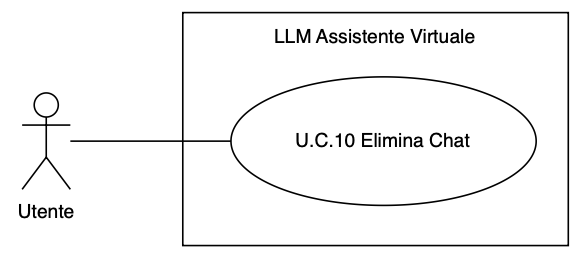
\includegraphics[width=0.7\textwidth]{img/UC10.png}
    \caption{U.C.10: Creazione di un nuovo template}
\end{figure}
\newpage

\subsubsection{U.C.11: Modifica di un template esistente}
\begin{itemize}
    \item \textbf{Attore}: Admin
    \item \textbf{Precondizioni}: L'amministratore ha effettuato l'accesso e ha selezionato un \href{https://code7crusaders.github.io/docs/RTB/documentazione_interna/glossario.html#template}{template\textsuperscript{G}} esistente dalla lista.
    \item \textbf{Postcondizioni}: Il \href{https://code7crusaders.github.io/docs/RTB/documentazione_interna/glossario.html#template}{template\textsuperscript{G}} selezionato viene aggiornato con i nuovi dati forniti.
    \item \textbf{Scenario principale}: L'amministratore visualizza l'elenco dei \href{https://code7crusaders.github.io/docs/RTB/documentazione_interna/glossario.html#template}{template\textsuperscript{G}} disponibili e seleziona quello che desidera modificare. Accede quindi ai dettagli del \href{https://code7crusaders.github.io/docs/RTB/documentazione_interna/glossario.html#template}{template\textsuperscript{G}}, dove può modificare sia la domanda predefinita che la risposta associata. Dopo aver apportato le modifiche necessarie, l'amministratore salva i cambiamenti, aggiornando così il \href{https://code7crusaders.github.io/docs/RTB/documentazione_interna/glossario.html#template}{template\textsuperscript{G}} nel sistema. Le modifiche apportate sono immediatamente visibili agli utenti quando utilizzano la funzione di selezione delle domande predefinite. 
    \item \textbf{Generalizzazioni}: -
    \item \textbf{Estensioni}: U.C.13
    \item \textbf{Inclusione}: -
\end{itemize}
\begin{figure}[H]
    \centering
    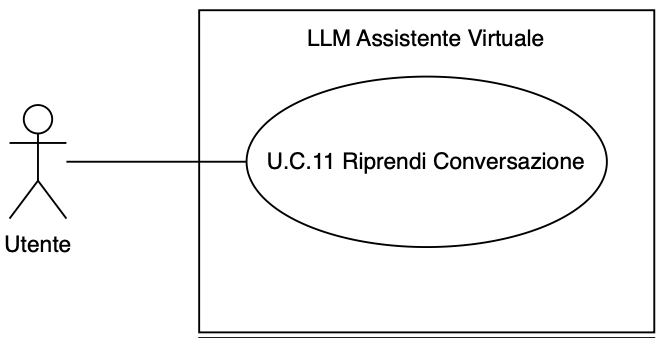
\includegraphics[width=0.7\textwidth]{img/UC11.png}
    \caption{U.C.11: Modifica di un template esistente}
\end{figure}
\newpage

\subsubsection{U.C.12: Elimina un template esistente}
\begin{itemize}
    \item \textbf{Attore}: Admin
    \item \textbf{Precondizioni}: L'amministratore ha effettuato l'accesso e ha selezionato un \href{https://code7crusaders.github.io/docs/RTB/documentazione_interna/glossario.html#template}{template\textsuperscript{G}} esistente dalla lista. 
    \item \textbf{Postcondizioni}: Il \href{https://code7crusaders.github.io/docs/RTB/documentazione_interna/glossario.html#template}{template\textsuperscript{G}} viene eliminato dal sistema e non è più disponibile per gli utenti.
    \item \textbf{Scenario principale}: L'amministratore, dalla lista dei \href{https://code7crusaders.github.io/docs/RTB/documentazione_interna/glossario.html#template}{template\textsuperscript{G}}, individua quello che intende eliminare. Dopo aver selezionato il \href{https://code7crusaders.github.io/docs/RTB/documentazione_interna/glossario.html#template}{template\textsuperscript{G}}, conferma l'operazione tramite un'apposita finestra di dialogo. Il sistema procede quindi a rimuovere il \href{https://code7crusaders.github.io/docs/RTB/documentazione_interna/glossario.html#template}{template\textsuperscript{G}}, aggiornando l'elenco dei \href{https://code7crusaders.github.io/docs/RTB/documentazione_interna/glossario.html#template}{template\textsuperscript{G}} disponibili. Da quel momento, la domanda predefinita associata non sarà più accessibile agli utenti.
    \item \textbf{Generalizzazioni}: -
    \item \textbf{Estensioni}: -
    \item \textbf{Inclusione}: -
\end{itemize}
\begin{figure}[H]
    \centering
    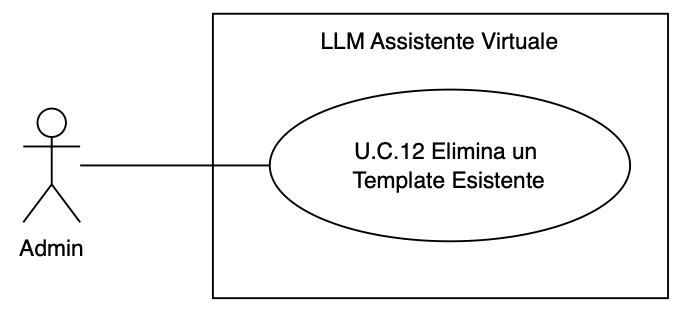
\includegraphics[width=0.7\textwidth]{img/UC12.png}
    \caption{U.C.12: Elimina un template esistente}
\end{figure}
\newpage

\subsubsection{U.C.13 Controllo Validità Formato}
\begin{itemize}
    \item \textbf{Attore}: Admin
    \item \textbf{Precondizioni}: L'amministratore sta creando o modificando un \href{https://code7crusaders.github.io/docs/RTB/documentazione_interna/glossario.html#template}{template\textsuperscript{G}}, ma inserisce un formato non valido (ad esempio, una domanda vuota o una risposta eccessivamente lunga ecc..)
    \item \textbf{Postcondizioni}: Il sistema non consente di salvare il \href{https://code7crusaders.github.io/docs/RTB/documentazione_interna/glossario.html#template}{template\textsuperscript{G}} e informa l'amministratore dell'errore.
    \item \textbf{Scenario principale}: Durante la creazione o modifica di un \href{https://code7crusaders.github.io/docs/RTB/documentazione_interna/glossario.html#template}{template\textsuperscript{G}}, l'amministratore inserisce dati non conformi, come una domanda lasciata vuota o una risposta con caratteri non consentiti. Il sistema esegue un controllo sui dati inseriti e rileva l'errore, bloccando il salvataggio del \href{https://code7crusaders.github.io/docs/RTB/documentazione_interna/glossario.html#template}{template\textsuperscript{G}}. Viene visualizzato un messaggio di errore chiaro che spiega il problema e invita l'amministratore a correggere i dati prima di procedere con il salvataggio.
    \item \textbf{Generalizzazioni}: -
    \item \textbf{Estensioni}: -
    \item \textbf{Inclusione}: -
\end{itemize}
\begin{figure}[H]
    \centering
    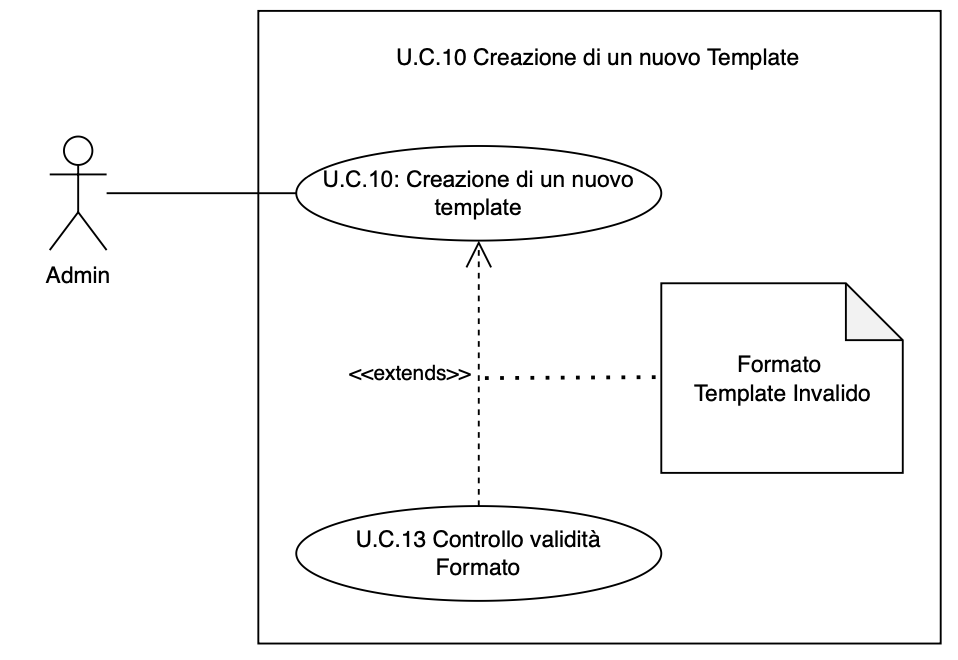
\includegraphics[width=0.6\textwidth]{img/UC13.1.png}
    %\caption{U.C.13 Controllo Validità Formato}
\end{figure}
\begin{figure}[H]
    \centering
    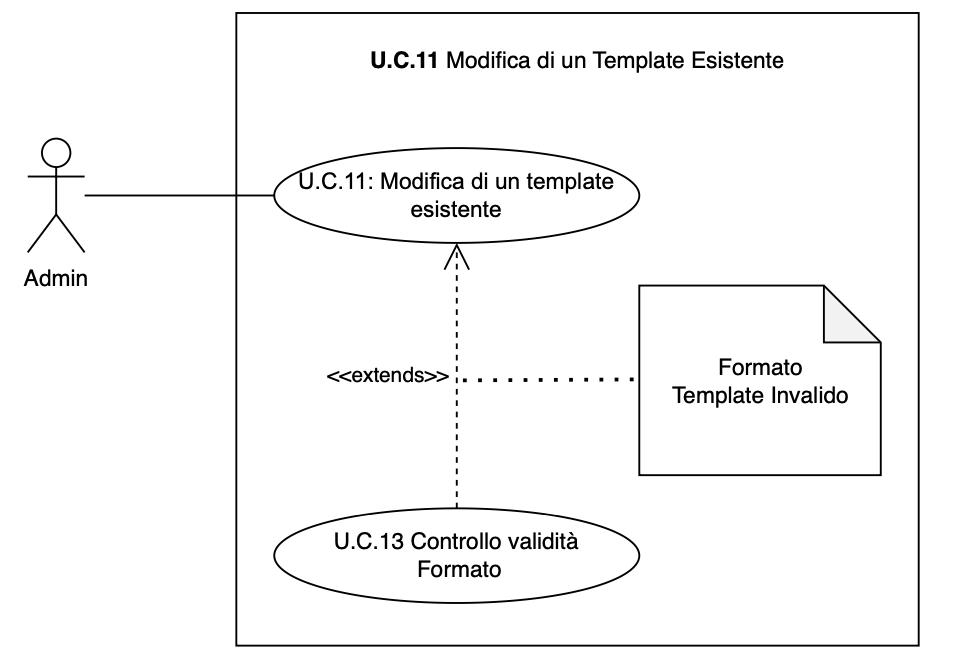
\includegraphics[width=0.6\textwidth]{img/UC13.2.png}
    \caption{U.C.13 Controllo Validità Formato}
\end{figure}
\newpage

\subsubsection{U.C.14: Visualizzazione delle metriche generali}
\begin{itemize}
    \item \textbf{Attore}: Admin
    \item \textbf{Precondizioni}: L'amministratore ha effettuato l'accesso alla dashboard di monitoraggio.
    \item \textbf{Postcondizioni}: L'amministratore visualizza le metriche principali del sistema.
    \item \textbf{Scenario principale}: L'amministratore seleziona l'opzione per visualizzare le statistiche generali e consulta i dati per analizzare le prestazioni del sistema.
    \item \textbf{Generalizzazioni}: -
    \item \textbf{Estensioni}: -
    \item \textbf{Inclusione}: -
\end{itemize}
\begin{figure}[H]
    \centering
    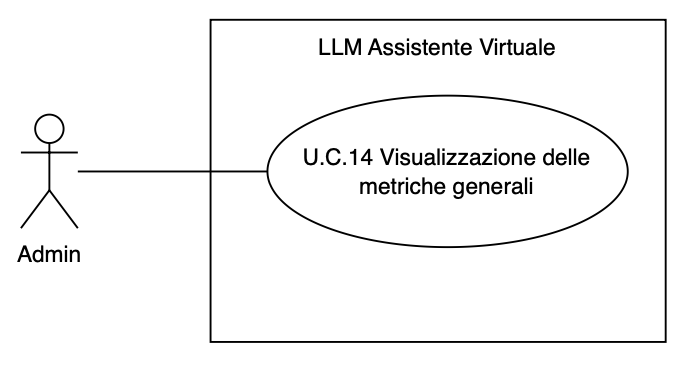
\includegraphics[width=0.7\textwidth]{img/UC14.png}
    \caption{U.C.14: Visualizzazione delle metriche generali}
\end{figure}
\newpage

\subsubsection{U.C.15: Visualizzazione Feedback Utenti}
\begin{itemize}
    \item \textbf{Attore}: Admin
    \item \textbf{Precondizioni}: L'amministratore ha effettuato l'accesso e ha selezionato la sezione relativa ai feedback degli utenti.
    \item \textbf{Postcondizioni}: I feedback degli utenti sulle risposte del chatbot sono stati visualizzati e analizzati.
    \item \textbf{Scenario principale}:  L'amministratore accede alla sezione dei feedback, consulta i giudizi degli utenti e utilizza le informazioni per migliorare il sistema.
    \item \textbf{Generalizzazioni}: -
    \item \textbf{Estensioni}: -
    \item \textbf{Inclusione}: -
\end{itemize}
\begin{figure}[H]
    \centering
    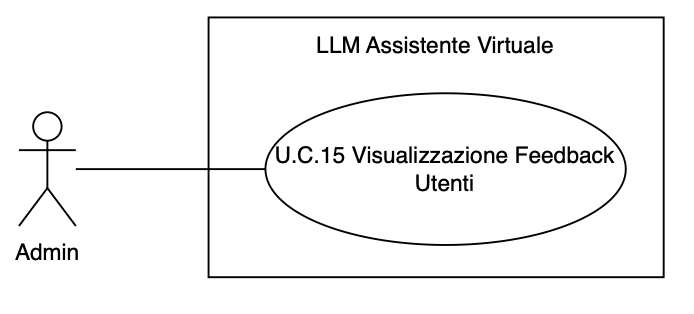
\includegraphics[width=0.7\textwidth]{img/UC15.png}
    \caption{U.C.15: Visualizzazione Feedback Utenti}
\end{figure}
\newpage

\subsubsection{U.C.16: Importazione di Dati}
\begin{itemize}
    \item \textbf{Attore}: Admin
    \item \textbf{Attore Secondario}: OpenAi
    \item \textbf{Precondizioni}: L'amministratore ha selezionato un file di dati da importare.
    \item \textbf{Postcondizioni}: I dati vengono caricati per la validazione.
    \item \textbf{Scenario principale}: L'amministratore seleziona il file dal proprio dispositivo e avvia il processo di importazione. Il sistema prepara i dati per la validazione.
    \item \textbf{Generalizzazioni}: -
    \item \textbf{Estensioni}: U.C.16.1
    \item \textbf{Inclusione}: -
\end{itemize}
\begin{figure}[H]
    \centering
    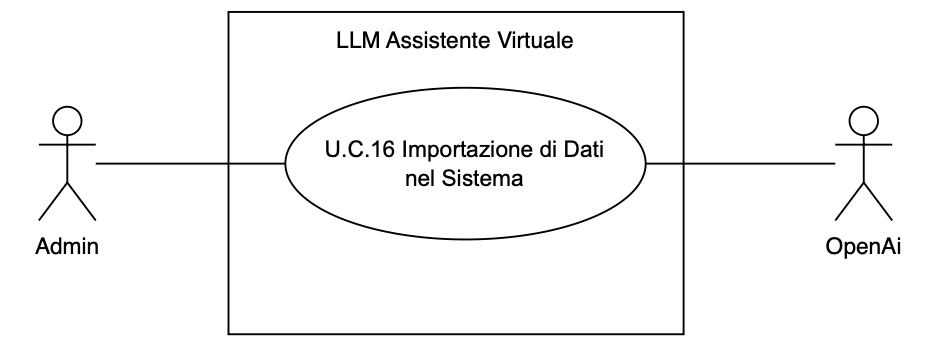
\includegraphics[width=0.8\textwidth]{img/UC16.png}
    \caption{U.C.16: Importazione di Dati}
\end{figure}
\newpage

\subsubsection{U.C.16.1: Validazione Formato}
\begin{itemize}
    \item \textbf{Attore}: Admin
    \item \textbf{Precondizioni}: L’amministratore vuole caricare un file dati da caricare.
    \item \textbf{Postcondizioni}: I file vengono respinti se il formato dati è sbagliato, altrimenti vengono importati.
    \item \textbf{Scenario principale}: Il sistema analizza il file, controlla la coerenza e il formato dei dati, se incoerente respinge e segnala errore.
    \item \textbf{Generalizzazioni}: -
    \item \textbf{Estensioni}: -
    \item \textbf{Inclusione}: -
\end{itemize}
\begin{figure}[H]
    \centering
    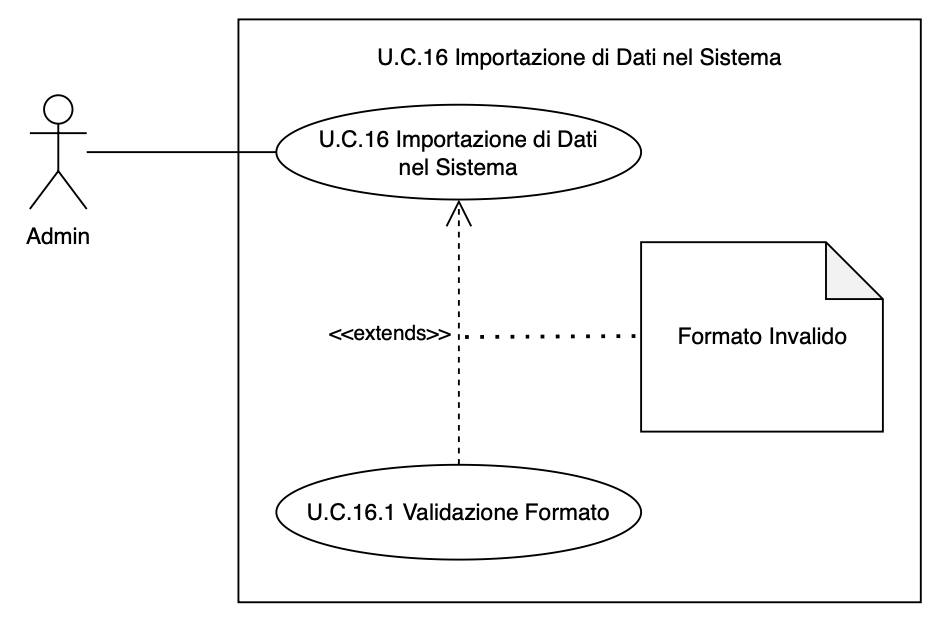
\includegraphics[width=0.7\textwidth]{img/UC16.1.png}
    \caption{U.C.16.1: Validazione Formato}
\end{figure}
\newpage

\subsubsection{U.C.17 Esportazione di Dati nel Sistema}
\begin{itemize}
    \item \textbf{Attore}: Admin
    \item \textbf{Precondizioni}: L’amministratore vuole esportare un file dati.
    \item \textbf{Postcondizioni}: I dati vengono esportati.
    \item \textbf{Scenario principale}: L'amministratore seleziona il file del database e avvia il processo di esportazione.
    \item \textbf{Generalizzazioni}: -
    \item \textbf{Estensioni}: -
    \item \textbf{Inclusione}: -
\end{itemize}
\begin{figure}[H]
    \centering
    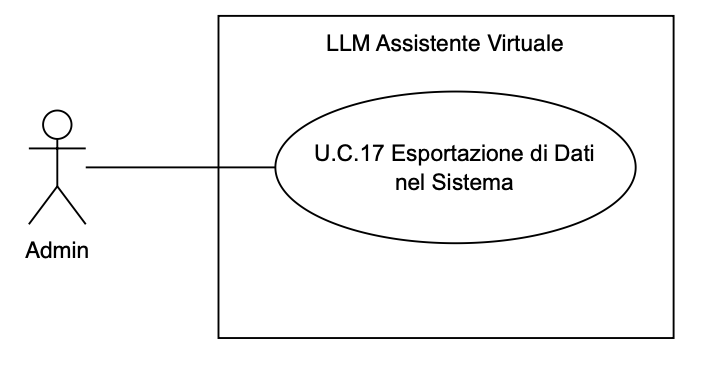
\includegraphics[width=0.7\textwidth]{img/UC17.png}
    \caption{U.C.17 Esportazione di Dati nel Sistema}
\end{figure}
\newpage

\subsubsection{U.C.18 Elimina Chat}
\begin{itemize}
    \item \textbf{Attore}: Utente
    \item \textbf{Precondizioni}: L'utente ha effettuato l'accesso ed è presente almeno una conversazione salvata.
    \item \textbf{Postcondizioni}: La conversazione selezionata viene eliminata dal sistema.
    \item \textbf{Scenario principale}: L'utente accede all'elenco delle chat salvate, seleziona una conversazione specifica e conferma l'eliminazione.
    \item \textbf{Generalizzazioni}: -
    \item \textbf{Estensioni}: -
    \item \textbf{Inclusione}: -
\end{itemize}
\begin{figure}[H]
    \centering
    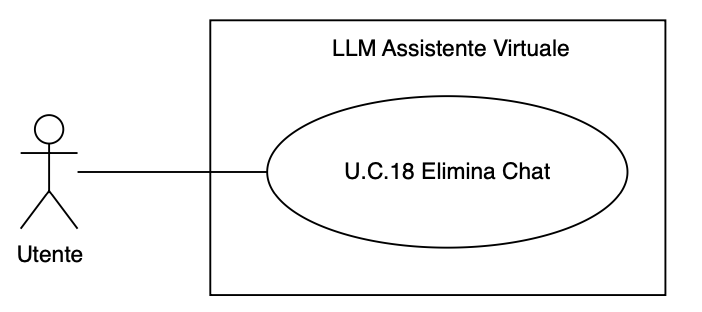
\includegraphics[width=0.7\textwidth]{img/UC18.png}
    \caption{U.C.18 Elimina Chat}
\end{figure}
\newpage

\subsubsection{U.C.19: Riprendi Conversazione}
\begin{itemize}
    \item \textbf{Attore}: Utente
    \item \textbf{Precondizioni}: L’utente ha effettuato l’accesso al sistema ed effettuato una conversazione
    \item \textbf{Postcondizioni}: L’utente riprende la conversazione con l’assistente virtuale.
    \item \textbf{Scenario principale}: L’utente ha per qualche motivo dovuto interrompere la conversazione e la riprende successivamente in un secondo momento.
    \item \textbf{Generalizzazioni}: -
    \item \textbf{Estensioni}: -
    \item \textbf{Inclusione}: -
\end{itemize}
\begin{figure}[H]
    \centering
    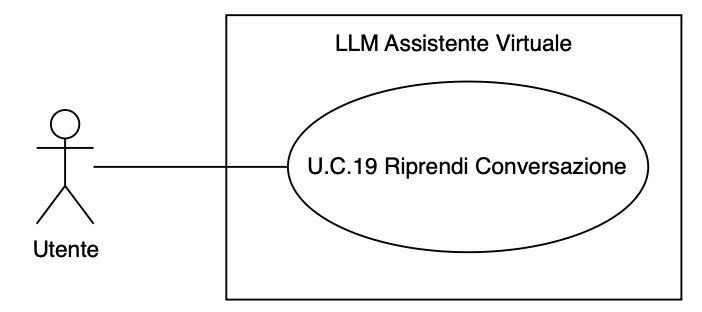
\includegraphics[width=0.7\textwidth]{img/UC19.png}
    \caption{U.C.19: Riprendi Conversazione}
\end{figure}
\newpage

\subsubsection{U.C.20: Risposta alla Richiesta dall’Amministratore}
\begin{itemize}
    \item \textbf{Attore}: Admin
    \item \textbf{Precondizioni}: L’amministratore ha effettuato l’accesso al sistema e in seguito alla dashboard per la gestione delle richieste di contatto. È presente almeno una richiesta inviata da un utente.
    \item \textbf{Postcondizioni}: L’amministratore ha risposto alla richiesta tramite email.
    \item \textbf{Scenario principale}: L’amministratore accede alla dashboard, seleziona una richiesta da gestire e ne visualizza i dettagli. Compone una risposta e la invia tramite il sistema.
    \item \textbf{Generalizzazioni}: -
    \item \textbf{Estensioni}: -
    \item \textbf{Inclusione}: -
\end{itemize}
\begin{figure}[H]
    \centering
    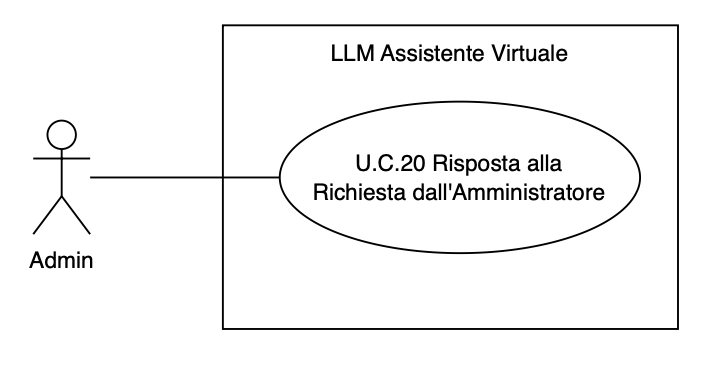
\includegraphics[width=0.7\textwidth]{img/UC20.png}
    \caption{U.C.20: Risposta alla Richiesta dall’Amministratore}
\end{figure}
\newpage

\subsubsection{U.C.21: Cambio stato Richiesta}
\begin{itemize}
    \item \textbf{Attore}: Admin
    \item \textbf{Precondizioni}: L’amministratore ha effettuato l’accesso al sistema e in seguito alla dashboard per la gestione delle richieste di contatto. È presente almeno una richiesta inviata da un utente.
    \item \textbf{Postcondizioni}: La richiesta è stata aggiornata come "gestita" dallo stato di “attesa”.
    \item \textbf{Scenario principale}: Dopo la risposta L’amministratore può decidere se lasciare la richiesta in stato di attesa o segnarla come “gestita”.
    \item \textbf{Generalizzazioni}: -
    \item \textbf{Estensioni}: -
    \item \textbf{Inclusione}: -
\end{itemize}
\begin{figure}[H]
    \centering
    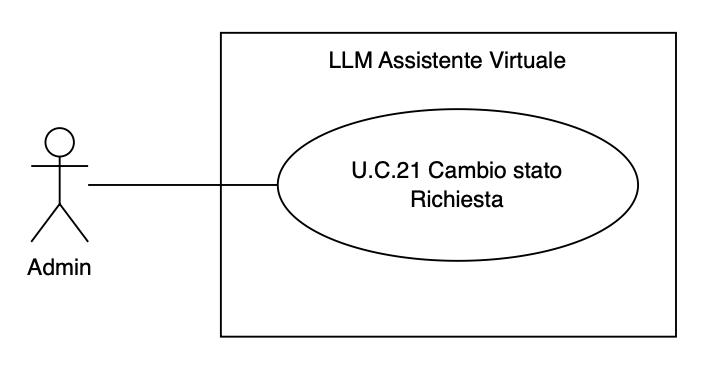
\includegraphics[width=0.7\textwidth]{img/UC21.png}
    \caption{U.C.21: Cambio stato Richiesta}
\end{figure}
\newpage

%% caso 21
\subsubsection{U.C.22 Invio Richiesta a un Operatore Umano}
\begin{itemize}
    \item \textbf{Attore}: Utente
    \item \textbf{Precondizioni}: L’utente ha ricevuto una risposta non soddisfacente dal sistema basato su \href{https://code7crusaders.github.io/docs/RTB/documentazione_interna/glossario.html#llm-large-language-model}{\textit{LLM}\textsuperscript{G}}.
    \item \textbf{Postcondizioni}: La richiesta dell’utente è stata inviata agli amministratori ed è visibile nella dashboard.    .
    \item \textbf{Scenario principale}: L’utente seleziona l’opzione per richiedere assistenza a un operatore umano, compila un modulo opzionale con eventuali dettagli e invia la richiesta. Il sistema registra la richiesta e la rende disponibile nella dashboard degli amministratori.
    \item \textbf{Generalizzazioni}: -
    \item \textbf{Estensioni}: -
    \item \textbf{Inclusione}: -
\end{itemize}
\begin{figure}[H]
    \centering
    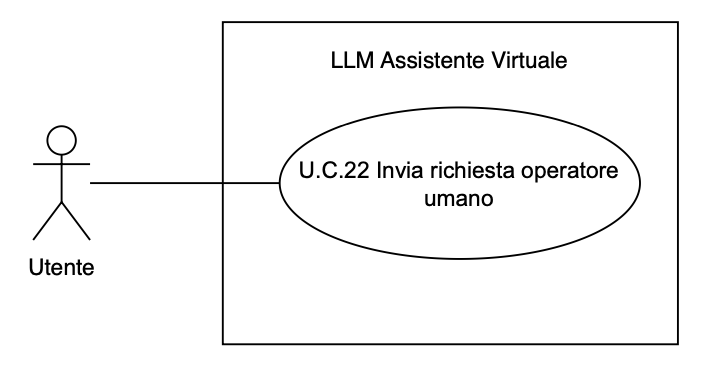
\includegraphics[width=0.7\textwidth]{img/UC22.png}
    \caption{U.C.22 Invio Richiesta a un Operatore Umano}
\end{figure}
\newpage